\begin{subsection}{Niveles}
  Los niveles del juego no serán secuenciales. El jugador puede acceder a ellos mediante un menú en el que se muestran personajes relacionados con la guerra del pacífico. Cada uno de estos personajes, tendrá asociada una \textit{línea del tiempo}, que contendrá un conjunto de niveles que el jugador puede jugar, sin que sea necesario pasarlos en ningún orden en especial, pero que están colocados en un orden descendente, de acuerdo al tiempo en el que se desarrollaron los sucesos.
  
  Sólamente se desarrollarán 2 niveles importantes, pero si el tiempo alcanza, se desarrollará uno más. A continuación, se describirán algunos niveles que no serán implementados, los niveles que sí serán implementados serán descritos con mayor detalle, y marcados con la etiqueta \indispensable, que indica que la característica es indispnsable, el resto, se marcará con la etiqueta \talvez, que indica que la característica se desarrollará sólamente si alcanza el tiempo.

  Los niveles se listan a continuación:

  \paragraph{Protagonista: } Ladislao Cabrera, coronel de artillería que dirigió la defenza del puente Tópater, a pesar que su ejército de 128 voluntarios era superado en número y armas por el ejército enemigo.
  
  Este personaje cuenta con tres niveles, de los cuales uno es indispensable:

  \paragraph{Desventaja} \talvez Un nivel en el que se muestra el momento en el que Ladislao fue llamado a comandar la defenza del puente Tópater. En este nivel se muestra que la fuerza de defenza estaba en desventaja, y que solo contaban con 128 hombres, y algunas armas, algunas en buen estado, y otras improvisadas.

  \paragraph{Estrategia} \talvez De cómo se planificó la defenza del puente Topater junto con Eduardo Abaroa. Se destruyen los puentes de acceso a la ciudad para poder protegerla mejor.

  \begin{subsubsection}{Batalla del Topater}
  \indispensable Este nivel es indispensable.

  El jugador toma el control de Omar Quispe, un minero que trabajaba en las minas de Eduardo Abaroa.

  \begin{section}{Antecedentes}
  \begin{subsection}{Juegos Comerciales}
    \begin{subsubsection}{Age of Empires (saga)}
      Es un juego de estrategia en tiempo real, en el que el jugador puede recolectar recursos. Estos recursos son usados para construir edificios que sirven para construir unidades y mejorarlas. El jugador puede armar un ejército e invadir el imperio de otros jugadores, todo esto mientras avanza a través de las edades de la historia.
      
      A parte de poder ser jugado en modo de escaramusas, también se puede jugar en modo campaña; en el modo campaña, el jugador es guiado a través de la historia medieval, peleando batallas y conociendo a los personajes más influyentes de esa época. También se muestran ocasionalmente algunos videos que explican el trasfondo de cada misión.
    \end{subsubsection}

    \begin{subsubsection}{Caesar (saga)}
      Es un videojuego de simulación de ciudades en el que el jugador construye una ciudad tomando el papel del César en la antigua Roma.

      A diferencia de Age of Empires, el aspecto educativo es muy reducido, sin embargo, la lógica de construcción de ciudades es muy acertada históricamente.
    \end{subsubsection}

    \begin{subsubsection}{Valiant Hearths}
      Es un juego de puzzle/aventura basado en cartas enviadas durante “la gran guerra” (WWI). El jugador maneja a varios personajes en el transcurso del juego, entre ellos: Karl, uno de los muchos alemanes deportados de Francia, Karl es separado de su esposa e hijo. El jugador deberá usar sus habilidades para sobrevivir, explorar el área y resolver puzzles, todo esto mientras es parte activa de su entorno, explorando cómo era el mundo durante la gran guerra en 1914.

      El juego se centra más en la vida de las personas durante la gran guerra, y aunque narra parte de la historia mediante textos informativos antes de cada nivel, esta historia no es la parte central de este juego, sino la interacción entre las personas que vivieron dicha guerra, y la forma en la que vivían. \cite{webpage:ubisoft}
    \end{subsubsection}
  \end{subsection}

  \begin{subsection}{Juegos \textit{indie}}
    %% REF
    Existen varias(Owens y Safley, s.f.)(CommonSense, s.f.) páginas web que contiene una gran colección de videojuegos educativos de historia. Actualmente existen 126 juegos de historia indexados en el portal playing history \footnote{Cantidad consultada el 25 de agosto de 2015}(Owens y Safley, s.f.). 1 Debido a la gran cantidad, solo se tomarán en cuenta algunos de estos videojuegos.

    \begin{subsubsection}{1066: The Game}
      %% REF
      Es un juego de estrategia por turnos, cuya jugabilidad se asemeja al estilo de combate del juego Heroes of Might and Magic(Ubisoft, s.f.). El jugador dirige a diferentes batallones en diversas batallas, cada batalla, representa una de las batallas en la que los ingleses lucharon defendiendo su territorio de los enemigos que los asediaban durante 1066. Antes de cada combate, una animación describe
el contexto histórico de la batalla.
    \end{subsubsection}

  \end{subsection}
  \begin{subsection}{Edutainment}
    %% REF
    Pese a que a este proyecto le compete, más que nada, el edutainment en los videojuegos, he encontrado información muy valiosa en reseñas sobre todo tipo de edutainment, escritas por una gran comunidad entusiasta (CommonSense, s.f.) del uso de la tecnología en el salón de clases. Pese a que, gran parte de esta información proviene de reseñas sobre plataformas web basadas en texto y foros de debate, estas plataformas contienen ideas que podrían ser incluso más efectivas si se transmitieran explotando la interactividad, la popularidad y la experiencia inmersiva de un videojuego.

    \begin{subsubsection}{Historical Scene Investigation}
      Es una página web en la que los estudiantes pueden explorar los archivos de varios ``casos históricos'', luego de leer cartas, ver fotografías, y explorar todo tipo de ``evidencias'', deberán responder a varias preguntas planteadas, respecto al contexto, sucesos y modo de vida de la época. 

      Las respuestas a estas preguntas no siempre serán obvias, muchas veces estarán ocultas implícitamente en detalles que podrían pasar desapercibidos por los jugadores. Por esta razón, es necesario que el jugador explore la evidencia, y preste mucha atención a todos los pequeños detalles.(Swan y Hofer, s.f.) 

      Debido a que el jugador concluye la respuesta a las preguntas planteadas, es mucho más probable que el aprendizaje sea significativo.(CommonSense, s.f.)
    \end{subsubsection}

    \begin{subsubsection}{HistoryPin}
      Es una aplicación web, parecida a google maps, en la que los usuarios pue- den ``pinnear'' fotografías a un mapa, estos pines son descritos mediante un sistema de crowdsourcing, en el que los usuarios pueden añadir información sobre algún pin en específico, sin importar si la información es histórica o personal.(brendan.knowlton@historypin.org, s.f.)
    \end{subsubsection}

    \begin{subsubsection}{Idea of America}
      Es una página web dirigida a alumnos de pregrado. La idea es que los estu- diantes accedan a esta página, para aprender los principios del debate y diálogo, con el fin de aprender historia de una forma más didáctica, y con un enfoque orientado a la crítica y la autocrítica.(history.org, s.f.)
    \end{subsubsection}    
  \end{subsection}

  \begin{subsection}{Antecedentes Teóricos}
    \begin{subsubsection}{Juegos \textit{indie}}
      Durante la época del nacimiento de la NES, en el año 1983, desarrollar video- juegos era muy difícil, una de las causas, era que la tecnología de almacenamiento de datos no estaba tan avanzada como en la actualidad, así que los lenguajes de programación eran rudimentarios y difíciles de manejar. Los límites para los desarrolladores y diseñadores también eran estrechos, debido a la velocidad de las computadoras de esa época y a las limitantes en el uso de sprites. 

      Pero actualmente, el desarrollo de videojuegos se ha simplificado bastante. 

      En la actualidad, niños de 13 años pueden desarrollar videojuegos sencillo(Meyer, 2013), y a causa de esto ha nacido una nueva industria: la industria de video- juegos indie. 

      Consiste en equipos de desarrollo de videojuegos compuestos por personas que no pertenecen a ninguna corporación ``grande'' como Ubisoft o Microsoft. 

      Estos pequeños equipos de desarrolladores crean pequeños juegos que, pese a que no pueden competir en gráficos y calidad de desarrollo contra corporaciones gigantes especializadas en el desarrollo de videojuegos, muchas veces tienen un gameplay innovador, o conceptos que los lanzan al éxito, como fue el caso de Minecraft de la ex-empresa Mojang, que fue comprada por Microsoft en 2014. 

      Estos pequeños desarrolladores independientes, se hacen llamar a sí mismos: indie game developers, o como abreviatura: indies.
    \end{subsubsection}

    \begin{subsubsection}{Edutainment}
      Pese al pesimismo -justificado por investigaciones- que rodea a los video- juegos en los temas de salud, y sobre todo, en los temas de pedagogía, existen investigaciones más optimistas, que afirman que los videojuegos pueden ser usa- dos como un recurso educativo, si se seleccionan de forma adecuada. 

      El término edutainment es un juego de palabras entre education, que significa ``educación'' en inglés, y ``entertainment'' que significa ``entretenimiento'' en inglés. Tal vez el término ``edutrenimiento'' sería una buena traducción. 

      6Se define como edutainment a cualquier contenido o sistema que además de desarrollar alguna habilidad o dejar una enseñanza práctica en sus jugadores, también es divertido. 

      El término también se aplica a cualquier contenido o sistema que no ``haya sido creado'' para educar, así como para cualquiera que no ``haya sido creado'' para entretener, y por lo tanto son entretenidos pero accidentalmente educa- tivos, o son educativos pero accidentalmente entretenidos, o accidentalmente educativos y entretenidos.
    \end{subsubsection}

    \begin{subsubsection}{Videojuegos y psicología}
      Existe una gran controversia respecto a los videojuegos, algunos de los con- flictos son: ¿cuánto tiempo debería una persona permanecer frente a una pantalla? Los resultados de una investigación realizada durante el 2012 concluyó que los niños, durante la etapa pre-escolar, permanecían más tiempo del recomendado \footnote{Según recomendaciónes australianas aprobadas por la APA} frente a una pantalla (Hinkley, Salmon, Okely, Crawford, y K., 2012) 

      ¿hasta qué punto es un videojuego lo suficientemente real como para interfe- rir en las decisiones, iniciativas o salud física de una persona? una investigación conducida por Mary E. Ballard y J. Rose Wiest durante el 2006 intenta deter- minar los efectos de jugar Mortal Kombat en las respuestas cardiovasculares en una población masculina (Ballard y Wiest, 1996).
    \end{subsubsection}

    \begin{subsubsection}{Desarrollo de habilidades}
      Algunos videojuegos desarrollan habilidades visuales espaciales ya que en muchos se requiere que el jugador rote figuras en su mente (como tétris) e incluso, que memorice el mapa de un lugar, que identifique los puntos cardinales y se dirija a varios puntos, todo esto mientras debe prestar atención a eventos auditivos y permanece bajo cierto estrés, como en el caso de los shooters que tienen una modalidad de multijugador. 

      Quiroga et. al. afirman que es posible medir el factor g, un factor que mide la inteligencia, mediante juegos comerciales.( Angeles Quiroga y cols., 2015)
    \end{subsubsection}    
  \end{subsection}
\end{section}

    \paragraph{Jugabilidad básica} El campo de batalla es lineal: izquierda o derecha. Hay opciones de esconderse, pero el jugador debe darse cuenta rápidamente que no debería esconderse, sino pelear, porque de lo contrario, la conquista es inminente.

  Para darle al jugador la motivación de avanzar hacia la derecha, a lo largo del camino encontrará cuerpos inertes de los soldados muertos en batalla, tanto bolivianos como chilenos, que le darán \textit{loot}: nuevas armas, municiones \talvez, agua para su cantimplora y raciones.

  Los invasores van de derecha a izquierda, y la variedad de enemigos que existe debe ser lo suficientemente amplia, para que el jugador disfrute la libertad de decidir las armas que usará. Los enemigos deben ser lo suficientemente difíciles de matar, para que el jugador no pueda, bajo ninguna circunstancia, sobrevivir a la lucha de 6 de ellos simultáneamente \indispensable.
  
  La cantidad de soldados bolivianos muertos que el jugador encuentra a lo largo del camino, debe ser relacional a la dificultad que el jugador experimente al luchar contra los enemigos que \textit{spawnean} a la derecha, en la siguiente batalla.
  
  El jugador deberá administrar correctamente su energía y vida para poder evitar el paso de la mayor cantidad posible de enemigos. Ya que el jugador puede decidir si luchar o no, debe existir un incentivo al finalizar el nivel luchando. Este incentivo será una \textit{pregunta}.

  \paragraph{Script} El jugador comienza en la ciudad, el coronel Ladislao está allí, hablando a las tropas desde una pila de sacos llenas con piedras de río construidas a modo de trinchera. Los soldados pareccen desmoralizados, están todos con sus cabezas abajo, el miedo y la tristeza pueden sentirse.

\textsc{[Ladislao Cabrera]} Hoy es nuestro día. Hoy la patria nos ha convocado a defender...

\textsc{[Ladislao Cabrera]} Hemos destruido los puentes para que el enemigo no pueda atravezar el río...

\textsc{[Ladislao Cabrera]} Eso nos da un poco de ventaja...

*algunos soldados (pocos) levantan  su cabeza*

\textsc{[Ladislao Cabrera]} Abaroa y otros compatriotas nos cubrirán por la retaguardia, nosotros iremos al frente.

*Omar Quispe levanta su cabeza al escuchar el nombre de Abaroa*

\textsc{[Ladislao Cabrera]} No dejéis que pasen! Esta es nuestra tierra, y la defenderemos con nuestra vida, no es así?.

*otros soldados más levantan su cabeza, algunos gritan ¡así es!*  

\textsc{[Ladislao Cabrera]} Somos bolivianos, y no preguntamos ``cuántos son?'' antes de defender a nuestra patria...

*los que aún estaban con su cabeza abajo, levantan su cabeza, todos los soldados gritan ¡así es! con el puño en alto*

\textsc{[Ladislao Cabrera]} AHORA A DEFENDER EL TOPATER! POR BOLIVIA!! *corre hacia la derecha, con su fusil en alto*.

*todos los soldados corren hacia la derecha, siguiendo a Ladislao, con sus armas en alto mientras gritan ¡POR BOLIVIA! seguido de un ilegible grito de guerra, dejando atrás a Omar Quispe.*

En este momento, el jugador puede comenzar a jugar, y toma el control de Omar Quispe.

  \paragraph{Mecanismos}

\paragraph{Especificaciones iniciales}
\begin{itemize}
  \item \textbf{Mecanismos del jugador}
  \begin{itemize} % mecanismos

  \item \textbf{Energía} \indispensable (o stámina) Es un atributo del personaje manejado por el jugador.
    
    \begin{itemize} % energía
    \item \indispensable Cada acción cuesta una cantidad de energía.
    \item \indispensable Si el jugador no tiene suficiente energía, no puede realizar la acción.
    \item \indispensable Se puede recuperar en un 50\%, instantáneamente, al realizar exitosamente la acción de tomar agua de la cantimplora.
    \item \talvez Se puede recuperar en un 5\% por minuto, al caminar.
    \item \talvez Se puede recuperar en un 10\% por minuto, al permanecer de pie.
    \item \talvez Se puede recuperar en un 20\% por minuto, al permanecer agachado e inmovil.
    \item \talvez Dentro de más baja sea la energía del jugador, todos los \textit{cooldowns}, \textit{casteos} se incrementarán, y el jugador será más lento al caminar y correr.
    \end{itemize} % energía

  \item \textbf{Vida} \indispensable (o HP) Es un atributo de todos los personajes.

    \begin{itemize} % vida
    \item \indispensable Un personaje controlado por el jugador, puede recuperar su HP en un 10\% cada minuto, después de haber realizado exitosamente la acción de comer una ración. Este efecto dura 9 minutos.

    \item \talvez Un personaje controlado por el jugador, puede recuperar en un 25\% cada minuto, después de haber realizado exitosamente la acción de primeros auxilios. Este efecto dura 5 minutos, y es anulado si el personaje recibe daño.

    \item \indispensable Cuando un atacante realiza exitosamente la acción de ataque contra un personaje, el HP del personaje se decrementará en función a los \textit{stats} del atacante.
    \end{itemize} %vida
  \end{itemize}

  \item \textbf{Armas} \indispensable Las armas son objetos que el jugador puede llevar sin límite en su inventario. Al ser seleccionadas, el jugador puede atacar con ellas, realizando una acción de ataque. El personaje solo puede equipar un arma a la vez, y si quiere cambiar, permanecerá inmovil durante un tiempo, simulando desempacar el arma nueva y guardar la anterior.

  \begin{itemize}
  \item \textbf{Casteo} \talvez El tiempo que el personaje debe esperar antes de que el ataque se realice. Algunas armas permiten permanecer cargadas sin desencadenar el ataque (como un rifle), pero otras no (como la picota).

  \item \textbf{Recarga} \talvez El tiempo que el personaje permanecerá inmóvil después de haber realizado el ataque.

  \item \textbf{Daño} \indispensable Determina el daño que hace a los HPs del oponente al ser realizada exitosamente la acción de ataque.

  \item \textbf{Dificultad} \indispensable Determina el costo en energía que el arma necesita para que el jugador realice una acción de ataque.
  \end{itemize}

  \item \textbf{Enemigos} \indispensable Son personajes que \textit{spawnean} inteligentemente del lado derecho de la pantalla, cuyo objetivo es cruzar al lado izquierdo de la pantalla. Pero si el jugador les hace daño, su objetivo cambia a causar que el HP del jugador caiga a cero.

  \begin{itemize}
  \item \textbf{Vida} (o HP) \indispensable
  \item \textbf{Agilidad} \talvez Determina la rapidez con la que se mueve y ataca el enemigo.
  \item \textbf{Fuerza} \indispensable Determina el daño que hace a los HPs del oponente al ser realizada exitosamente la acción de ataque.
  \end{itemize}

  Estos tres mecanismos crean dos campos de decisión: (agilidad, vida) y (fuerza, vida).

\end{itemize}


\paragraph{Lista de enemigos}

\begin{itemize}
\item \textbf{Milicia}
  \begin{center}
    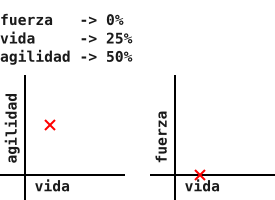
\includegraphics[width=.3\textwidth]{assets/lvl-design/milicia.png}
  \end{center}

\item \textbf{Caballería}
  \begin{center}
    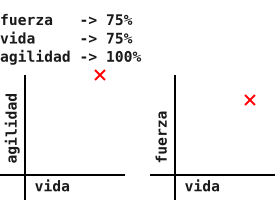
\includegraphics[width=.3\textwidth]{assets/lvl-design/caballeria.png}
  \end{center}

\item \textbf{Soldado}
  \begin{center}
    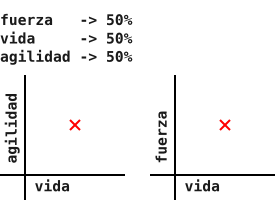
\includegraphics[width=.3\textwidth]{assets/lvl-design/soldado.png}
  \end{center}

\item \textbf{Artillero}
  \begin{center}
    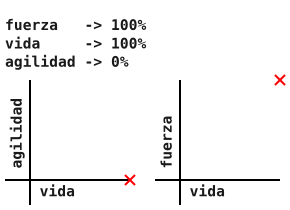
\includegraphics[width=.3\textwidth]{assets/lvl-design/artillero.png}
  \end{center}
\end{itemize}

\paragraph{Lista de armas}

\begin{itemize}
\item \textbf{Picota}
  
  \begin{center}
    \begin{tabular}{c|c}
      \textbf{Fortalezas} & \textbf{Debilidades} \\
      \hline
      Artillero & Caballería \\
      & Soldado
    \end{tabular}
  \end{center}

  \begin{center}
    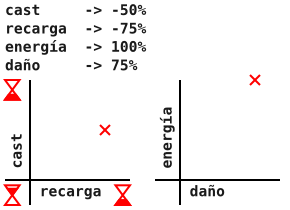
\includegraphics[width=.35\textwidth]{assets/lvl-design/picota.png}
  \end{center}

\item \textbf{Lanza} Eficaz contra caballería.

  \begin{center}
    \begin{tabular}{c|c}
      \textbf{Fortalezas} & \textbf{Debilidades} \\
      \hline
      Caballería & Soldado \\
      & Artillero
    \end{tabular}
  \end{center}

  \begin{center}
    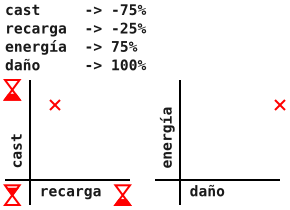
\includegraphics[width=.35\textwidth]{assets/lvl-design/lanza.png}
  \end{center}

\item \textbf{Oz}

  \begin{center}
    \begin{tabular}{c|c}
      \textbf{Fortalezas} & \textbf{Debilidades} \\
      \hline
      Milicia & Artillero
    \end{tabular}
  \end{center}

  \begin{center}
    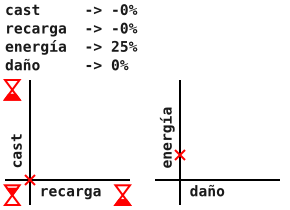
\includegraphics[width=.35\textwidth]{assets/lvl-design/oz.png}
  \end{center}

\item \textbf{Fusil}
  

  \begin{center}
    \begin{tabular}{c|c}
      \textbf{Fortalezas} & \textbf{Debilidades} \\
      \hline
      Caballería & Artillero \\
      Milicia & Munición limitada \\
      Soldado
    \end{tabular}
  \end{center}

  \begin{center}
    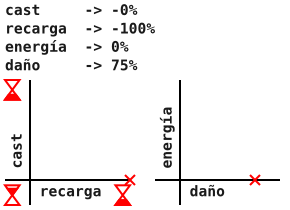
\includegraphics[width=.35\textwidth]{assets/lvl-design/fusil.png}
  \end{center}
\end{itemize}

    \paragraph{Diseño de niveles}

  \textit{Advertencia: }El arte usado para el diseño de niveles no es definitivo. Es solo una maqueta

  \paragraph{Especificaciones necesarias}

  \begin{itemize}

  \item \textbf{Duración }Al jugador debería tomarle 13 minutos pasar este nivel.
    \begin{itemize}
    \item \textbf{Batallas} El 60\% de este tiempo, debería tener enemigos presentes en la pantalla. (6 minutos)
    \item \textbf{Explorando} El 20\%, el jugador, probablemente, lo pase experimentando con los comandos, y observando detalles sin avanzar en el mapa. (2.25 minutos).
    \item \textbf{Caminando} El resto del tiempo (20\%), el jugador pasará, probablemente, avanzando hacia la derecha. (casi 6 minutos)
    \end{itemize}
  \item \textbf{Velocidad} Omar Quispe camina a una velocidad de $70\frac{px}{s}$
  \item \textbf{Longitud } Por lo tanto, el juego debería poder pasarse caminando, sin enemigos, en $(15)(60\%) = 9$ minutos. En vista de la velocidad de Omar Quispe, la longitud del juego debería ser de $d = vt = 70 * (9*60) = 10920 px$. Debido al diseño, se ajustó a $14520$ pixeles de largo.

  \item \textbf{Preguntas: }
    \begin{itemize}
    \item \textbf{¿Qué pasó con los caídos?} El jugador podrá desbloquear esta pregunta al encontrar soldados heridos a lo largo del camino e interactuar con ellos.
    \item \textbf{¿Sembradores en el desierto?} Esta pregunta se desbloquea mientras Ladislao está dando su discurso, el jugador podrá ver entre la milicia a algunos granjeros con azadas, las azadas son importantes porque implican que los granjeros no cuidan ganado, sino sembradíos.
    \item \textbf{¿Por qué era estratégicamente importante Calama?} Esta pregunta se desbloquea si el jugador logra sobrevivir hasta el final del nivel.
    \end{itemize}    

  \end{itemize}

  \paragraph{Nivel}

  En La parte inicial, el jugador permanece inmóvil, ya está equipado con una picota, y puede ver a sus compatriotas armados con armas improvisadas, algunos de ellos tienen fusiles.

  Aquí se desarrolla el script.
  \begin{center}
    \includegraphics[width=.9\textwidth]{../prototype/01.png}
  \end{center}

  En la parte inicial, se le enseña al jugador los controles básicos: caminar, correr, la mecánica de la energía y cómo recargarla, y la mecánica de la vida y cómo recargarla.
  \begin{center}
    \includegraphics[width=.9\textwidth]{../prototype/02.png}
  \end{center}


  En la primera batalla se le enseña cómo atacar y cubrirse. Un poco más adelante el jugador consigue la Oz, junto con la pregunta: ¿Sembradores en el desierto?, descubrirá que la oz es más rápida y consume menos energía, pero hace tan poco daño que es difícil acabar con los artilleros con ella. Decidirá si seguir usando su picota, o usar la oz, o una mezcla.
  \begin{center}
    \includegraphics[width=.9\textwidth]{../prototype/03.png}
  \end{center}

  El primer encuentro con la milicia, está diseñado para que el jugador recuerde el funcionamiento de la oz, e intente usarla de nuevo, dándose cuenta que es efectiva contra este tipo de enemigos, pero que la picota es muy difícil de usar contra blancos móviles.
  \begin{center}
    \includegraphics[width=.9\textwidth]{../prototype/04.png}
  \end{center}

  
  El primer encuentro con la caballería, está diseñado para que el jugador se de cuenta que puede esconderse de las batallas. Esta caballería es extremadamente difícil de derrotar con oz o con picota, pero no es imposible. El jugador puede decidir si esconderse, o luchar y terminar sumamente exhausto y herido.

  \begin{center}
    \includegraphics[width=.9\textwidth]{../prototype/05.png}
  \end{center}

  Más adelante, encontrará la lanza, que es ideal contra caballería. Luego, un campo abierto en el que no podrá esconderse, y deberá enfrentarse a la tropa montada con su lanza. Puede enfrentarlo con las otras armas, pero estará demasiado exhausto para hacerlo, así que será muy difícil.
  \begin{center}
    \includegraphics[width=.9\textwidth]{../prototype/06.png}
  \end{center}

  El resto del nivel, transcurre mezclando astutamente estos 4 diferentes tipos de enemigos para que el jugador haga uso de sus habilidades para derrotarlos.

  Y por último, el jugador debería asustarse al ver tantos soldados caídos, durante todo el nivel, la cantidad de soldados caídos es proporcional a la dificultad de la siguiente batalla.

  El jugador tiene la opción de esconderse, o de seguir. Debería darse cuenta que algo anda mal al ver algunos soldados caídos que parecían estar huyendo de la batalla, y más adelante, ve a 3 de ellos corriendo hacia el lado contrario, gritando ``retirada!''. El jugador también tiene la opción de huir, pero no deberá dejar que el fuego enemigo le llegue.x
  
  \begin{center}
    \includegraphics[width=.9\textwidth]{../prototype/07.png}
  \end{center}


  


\end{subsubsection}


\end{subsection}
